En este capítulo describimos el desarrollo de diversos códigos, escritos en el lenguaje de programación \Cpp{}, para facilitar el cálculo explícito de la topología de adyacencia y la topología de incidencia de un grafo finito, calculando, en cada caso, los abiertos subbásicos, los abiertos básicos y la colección de todos los abiertos de la topología en cuestión, recibiendo como entrada el número de vértices y la matriz de adyacencia del grafo que se desea estudiar. 
\section{Funciones preliminares}\label{sec:funciones_preliminares}
En esta sección describimos las funciones que se usarán conjuntamente para el cálculo de la topología de adyacencia y de la topología de incidencia. El objetivo grande que se desea con el grueso de funciones es lograr realizar intersecciones y uniones de conjuntos. Para esto nos apoyaremos fuertemente en el uso de matrices y vectores, y de las funcionalidades básicas que ofrece \Cpp{} para la manipulación de éstas.
Para la implementación de las funciones usamos cuatro cabeceras de la biblioteca estándar de \Cpp{}.
\begin{lstlisting}[caption={Encabezado del código}, label={cod:encabezado}]
#include <iostream>
#include <fstream>
#include <vector>
#include <cmath>
\end{lstlisting}
La cabecera \texttt{<iostream>} no es necesaria para imprimir texto en la terminal. La cabecera \texttt{<fstream>} la incluimos para poder leer archivos del tipo \texttt{.txt}, donde guardaremos el número de vértices y la matriz de adyacencia del grafo en cuestión. La cabecera \texttt{<vector>} nos permite la creación y manipulación de vectores y matrices. Por último, la cabecera \texttt{<cmath>} la implementamos para usar la función \texttt{pow}, con la cual realizamos la operación potencia de números enteros.\\\\
Para el funcionamiento del código usaremos archivos \texttt{.txt} para almacenar la información necesaria del grafo al que se le calcularán las topologías da adyacencia y de incidencia. Esta se conforma únicamente por un número entero que representa el número de vértices del grafo en cuestión, y un arreglo rectangular de ceros y unos, separados por \texttt{tabs} y renglones, que representa la matriz de adyacencia del mismo. Mostramos a continuación un par de ejemplos.
\begin{figure}[H]
   \centering
   % Fila 1: el grafo y el archivo, centrados verticalmente
   \begin{minipage}[c]{0.40\textwidth}
      \centering
      \resizebox{0.78\linewidth}{!}{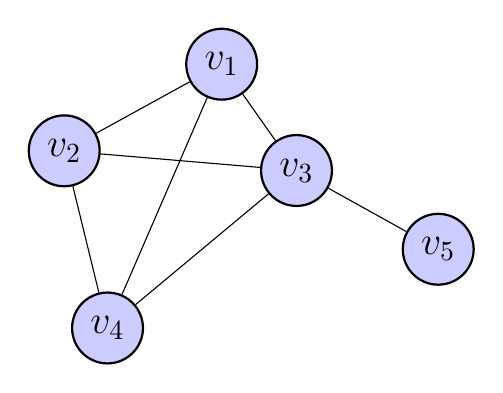
\begin{tikzpicture}[
  scale=1,
  vnode/.style={circle, fill=blue!20, draw=black, thick, minimum size=9mm, inner sep=0pt, font=\Large}
]
  % Vértices
  \node[vnode] (v1) at (2.0, 3.35) {$v_1$};
  \node[vnode] (v2) at (0.0, 2.25) {$v_2$};
  \node[vnode] (v3) at (2.95, 2.0) {$v_3$};
  \node[vnode] (v4) at (0.55, 0.0) {$v_4$};
  \node[vnode] (v5) at (4.75, 1.0) {$v_5$};

  % Aristas
  \foreach \from/\to in {v1/v2, v1/v3, v1/v4, v2/v3, v2/v4, v3/v4, v3/v5}
    \draw (\from) -- (\to);
\end{tikzpicture}
}
   \end{minipage}%
   \hspace{1.5em}%
   \begin{minipage}[c]{0.42\textwidth}
\begin{lstlisting}[framexrightmargin=-4.4pt]
5
0  1  1  1  0
1  0  1  1  0
1  1  0  1  1
1  1  1  0  0
0  0  1  0  0
\end{lstlisting}
   \end{minipage}

   % Fila 2: los pies, alineados arriba y centrados
   \captionsetup{format=plain, justification=centering}
   \begin{minipage}[t]{0.40\textwidth}
      \captionof{figure}{Grafo $G_1$}
      \label{fig:G_1}
   \end{minipage}%
   \hspace{1.5em}%
   \begin{minipage}[t]{0.42\textwidth}
      \captionof{lstlisting}{Archivo \texttt{1\_Mat\_Ady.txt} para guardar la información de $G_1$}
      \label{cod:1_Mat_Ady}
   \end{minipage}
\end{figure}

\begin{figure}[H]
   \centering
   % Fila 1: el grafo y el archivo, centrados verticalmente
   \begin{minipage}[c]{0.40\textwidth}
      \centering
      \resizebox{0.78\linewidth}{!}{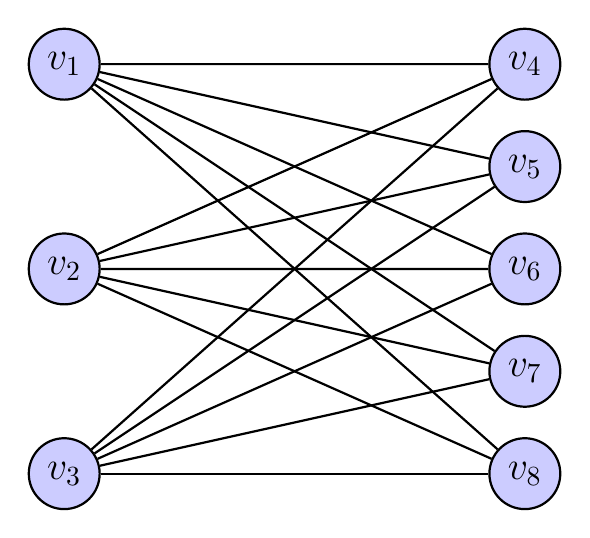
\begin{tikzpicture}[
  scale=1.3,
  vnode/.style={circle, fill=blue!20, draw=black, thick, minimum size=9mm, inner sep=0pt, font=\Large}
]
  % Partición izquierda
  \node[vnode] (v1) at (0, 4) {$v_1$};
  \node[vnode] (v2) at (0, 2) {$v_2$};
  \node[vnode] (v3) at (0, 0) {$v_3$};

  % Partición derecha
  \foreach \j in {4,...,8} {
    \node[vnode] (v\j) at (4.5, {8-\j}) {$v_{\j}$};
  }

  % Aristas: cada vértice de la izquierda con cada vértice de la derecha
  \foreach \i in {1,2,3} {
    \foreach \j in {4,...,8} {
      \draw[thick] (v\i) -- (v\j);
    }
  }
\end{tikzpicture}
}
   \end{minipage}%
   \hspace{1.5em}%
   \begin{minipage}[c]{0.42\textwidth}
\begin{lstlisting}[framexrightmargin=-4.4pt]
8 (*@\label{lin:r1_2_Mat_Ady}@*)
0 0 0 1 1 1 1 1 (*@\label{lin:inicio_2_Mat_Ady}@*)
0 0 0 1 1 1 1 1
0 0 0 1 1 1 1 1
1 1 1 0 0 0 0 0
1 1 1 0 0 0 0 0
1 1 1 0 0 0 0 0
1 1 1 0 0 0 0 0
1 1 1 0 0 0 0 0 (*@\label{lin:fin_2_Mat_Ady}@*)
\end{lstlisting}
\end{minipage}

   % Fila 2: los pies, alineados arriba y centrados
   \captionsetup{format=plain, justification=centering}
   \begin{minipage}[t]{0.40\textwidth}
      \captionof{figure}{Grafo $K_{3,5}$}
      \label{fig:K_3,5}
   \end{minipage}%
   \hspace{1.5em}%
   \begin{minipage}[t]{0.42\textwidth}
      \captionof{lstlisting}{Archivo \texttt{2\_Mat\_Ady.txt} para guardar la información de $K_{3,5}$}
      \label{cod:2_Mat_Ady}
   \end{minipage}
\end{figure}

Así, por ejemplo, en la \Cref{lin:r1_1_Mat_Ady} del \Cref{cod:1_Mat_Ady}, el número $5$ hace referencia al número de vectores del grafo $G_1$, mientras que la \Cref{lin:r1_2_Mat_Ady} del \Cref{cod:2_Mat_Ady} hace referencia al número de vértices del grafo $K_{3,5}$. Igualmente, en las \Crefrange{lin:inicio_1_Mat_Ady}{lin:fin_1_Mat_Ady} del \Cref{cod:1_Mat_Ady}, se representa la matriz de adyacencia
\begin{ceqn}
\[
\begin{pmatrix}
   0 & 1 & 1 & 1 & 0 \\
   1 & 0 & 1 & 1 & 0 \\
   1 & 1 & 0 & 1 & 1 \\
   1 & 1 & 1 & 0 & 0 \\
   0 & 0 & 1 & 0 & 0
\end{pmatrix}
\]
\end{ceqn}
del grafo $G_1$. Análogamente, en las líneas \Crefrange{lin:inicio_2_Mat_Ady}{lin:fin_2_Mat_Ady} del \Cref{cod:2_Mat_Ady}, se representa la matriz de adyacencia
\begin{ceqn}
\[
\begin{pmatrix}
   0 & 0 & 0 & 1 & 1 & 1 & 1 & 1 \\
   0 & 0 & 0 & 1 & 1 & 1 & 1 & 1 \\
   0 & 0 & 0 & 1 & 1 & 1 & 1 & 1 \\
   1 & 1 & 1 & 0 & 0 & 0 & 0 & 0 \\
   1 & 1 & 1 & 0 & 0 & 0 & 0 & 0 \\
   1 & 1 & 1 & 0 & 0 & 0 & 0 & 0 \\
   1 & 1 & 1 & 0 & 0 & 0 & 0 & 0 \\
   1 & 1 & 1 & 0 & 0 & 0 & 0 & 0
\end{pmatrix}
\]
\end{ceqn}
del grafo $K_{3,5}$.
\begin{lstlisting}[caption={Función \lstinline|leerMatriz|: lectura de la matriz de adyacencia desde un archivo}, label={cod:leerMatriz}]
std::vector<std::vector<bool>> leerMatriz(std::ifstream& file){
   int n;
   file >> n;
   std::vector<std::vector<bool>> Mat_Ady(n, std::vector<bool>(n));
   for(int i=0; i<=n-1; i++){
      for(int j=0; j<=n-1; j++){
         bool valor;
         file >> valor;
         Mat_Ady[i][j] = valor;
      }
   }
   return Mat_Ady;
}\end{lstlisting}

\section{Topología de adyacencia}\label{sec:adyacencia_computacional}
\section{Topología de incidencia}\label{sec:incidencia_computacional}
